% Valens Book II.22 Second example chart
\documentclass[border=10pt]{standalone}
% packages used by all the chart files
\usepackage{wasysym}	% for astrology symbols
\usepackage{starfont}		% astrology font
\usepackage{tikz}			% drawing package
\usetikzlibrary{backgrounds, calc, quotes}
\starfontsans

\tikzset{
	pics/fortune/.style ={ % Lot of Fortune
		code={
			\node (lot) [draw, circle, thick] {};
			\draw [thick] (lot.north east) -- (lot.south west)
    				(lot.north west) -- (lot.south east);}
	}
}

\tikzset{ % Lot of Daimon
	daimon/.pic ={ 
		\node (lot) [draw, circle, thick, font=\bfseries] {};
		\draw [very thick] ([yshift=0.05cm]lot.north) --
							 ([yshift=-0.05cm]lot.south);
	}
}

\tikzset{
	pics/lot/.style = { % Generic Lot with symbol parameter
			code={\node [draw, circle, thick, font=\bfseries, scale=0.5]
						 {\textbf{\textsl{#1}}};}
	}
}


\begin{document}
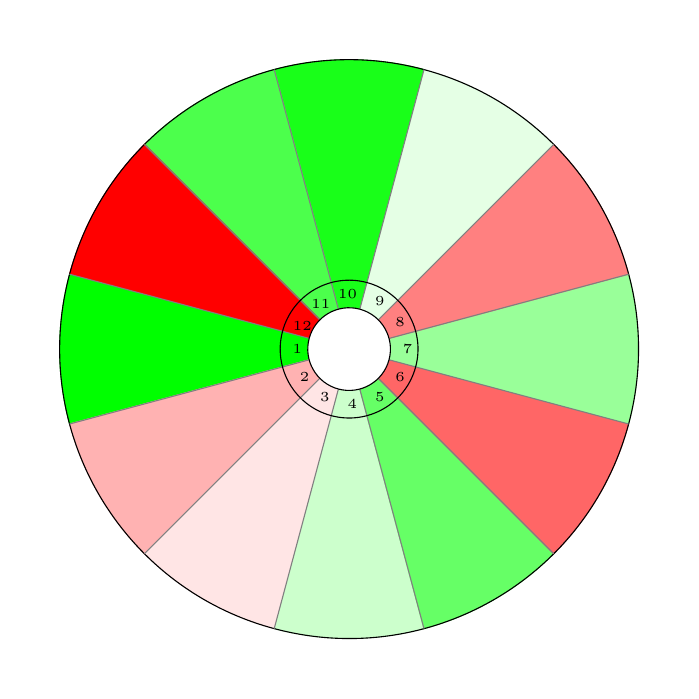
\begin{tikzpicture}[scale=3.5]
\begin{scope}[rotate=165]
	% draw numbered, fixed house positions
	\foreach \sign/\label in {
		0 / 1, 
		30/ 2, 
		60 / 3,
		90 / 4, 
		120 / 5, 
		150 / 6,
		180/ 7 , 
		210 / 8, 
		240 / 9,
		270 + 5 / 10, 
		300 + 5 / 11, 
		330 + 5/ 12}
	\draw (\sign + 15:0.2) node {\tiny\label};
\end{scope}

\begin{scope}[rotate=75]
	% --- Draw the basic chart
	% draw the circles
	\draw (0,0) circle(1.05);
	%\draw (0,0) circle(0.85);
	
	% draw cusps
	\foreach \x in {0,30,...,330} {
	        % lines from center to point
	        \draw[gray] (0,0) -- (\x:1.05);
	}
	
	% draw center of circle
	\fill[white] (0,0) circle(0.15);
	\draw (0,0) circle(0.15);
	\draw (0,0) circle(0.25);
	
	% draw sign labels
%	\foreach \sign/\label in {
%	15 /\Aries, 45 /\Taurus, 75 /\Gemini,
%	105 /\Cancer, 135 /\Leo, 165 /\Virgo,
%	195 /\Libra, 225 /\Scorpio, 255 /\Sagittarius,
%	285 /\Capricorn, 315 /\Aquarius, 345 /\Pisces}
%	\draw (\sign:0.95) node {\label};
	
	% --- draw Asc and MC lines
%	\draw [->, red] 
%	    (285:1.2)--(105:1.2cm)
%	    node [above] {\ASC}; % $ 0^\circ$};
	
	%\draw [->, blue, ultra thick] 
	 %   (195:1.2)--(15:1.2)node [left] {\MC}; %$ 10^\circ$};	
	
	% -- Colour house
	 % -- 	arc(start angle : delta angle : radius)
 	 \scoped[on background layer]\filldraw[green!90]
     	(0,0) -- (0:1.05) arc (0:30:1.05);	
 	 \scoped[on background layer]\filldraw[green!70]
     	(0,0) -- (30:1.05) arc (30:60:1.05);	     	
 	 \scoped[on background layer]\filldraw[green]
     	(0,0) -- (90:1.05) arc (90:120:1.05);
 	 \scoped[on background layer]\filldraw[green!20]
     	(0,0) -- (180:1.05) arc (180:210:1.05); 
 	 \scoped[on background layer]\filldraw[green!60]
     	(0,0) -- (210:1.05) arc (210:240:1.05);      	
 	 \scoped[on background layer]\filldraw[green!40]
     	(0,0) -- (270:1.05) arc (270:300:1.05);    
 	 \scoped[on background layer]\filldraw[green!10]
     	(0,0) -- (330:1.05) arc (330:360:1.05);      	 
     	
 	 \scoped[on background layer]\filldraw[red!10]
     	(0,0) -- (150:1.05) arc (150:180:1.05);    
 	 \scoped[on background layer]\filldraw[red!30]
     	(0,0) -- (120:1.05) arc (120:150:1.05);
 	 \scoped[on background layer]\filldraw[red!50]
     	(0,0) -- (300:1.05) arc (300:330:1.05);     	         	  	 
 	 \scoped[on background layer]\filldraw[red!60]
     	(0,0) -- (240:1.05) arc (240:270:1.05);     		
 	 \scoped[on background layer]\filldraw[red]
     	(0,0) -- (60:1.05) arc (60:90:1.05);
     		
	% --- draw planets
%	\node at (40:0.7)  [blue] {\LARGE\Sun};      
%	\node at (55:0.7)   {\Mercury};  
%	\node at (15:0.7) [blue] {\large\Moon};     
%	\node at (280:0.7) {\Jupiter}; 
%	\node at (95:0.7)  {\Saturn};   
%	\node at (105:0.7) [blue] {\large\Mars};     
%	\node at (115:.7) [blue]  {\Large\Venus};     	
%	\node at (75:0.7)  {\Fortune};

\end{scope}
\end{tikzpicture}
\end{document}
